\begin{pastexam}[label={px:ust-106-ee-ds-09}]{臺聯大電機類 106 學年度 第九題}
（問答）

(10\%) Please convert the following tree to a binary tree.

\begin{center}
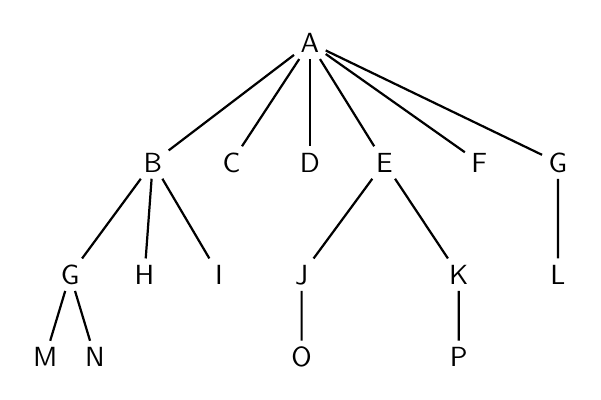
\begin{tikzpicture}[x=1.05cm,y=-0.95cm,every node/.style={font=\sffamily,inner sep=2pt},thick]
\node (A) at (4.4,0.7) {A};
\node (B) at (2.5,2.3) {B};
\node (C) at (3.45,2.3) {C};
\node (D) at (4.4,2.3) {D};
\node (E) at (5.3,2.3) {E};
\node (F) at (6.45,2.3) {F};
\node (G) at (7.4,2.3) {G};
\node (G2) at (1.5,3.8) {G};
\node (H) at (2.4,3.8) {H};
\node (I) at (3.3,3.8) {I};
\node (J) at (4.3,3.8) {J};
\node (K) at (6.2,3.8) {K};
\node (L) at (7.4,3.8) {L};
\node (M) at (1.2,4.9) {M};
\node (N) at (1.8,4.9) {N};
\node (O) at (4.3,4.9) {O};
\node (P) at (6.2,4.9) {P};
\foreach \c in {B,C,D,E,F,G} \draw (A) -- (\c);
\foreach \c in {G2,H,I} \draw (B) -- (\c);
\draw (G2) -- (M) (G2) -- (N) (E) -- (J) (E) -- (K) (J) -- (O) (K) -- (P) (G) -- (L);
\end{tikzpicture}
\end{center}
\end{pastexam}

\begin{pastsoln}
原圖有兩個節點都標成 G：一個是 A 的第六個子節點（底下有 L），一個是 B 的第一個子節點（底下有 M、N）。
它們是不同的節點，下面用「A 的子節點 G」「B 的子節點 G」區分。

用左孩子右兄弟表示法（資結書第~7.2.3~節）：每個節點的左指標指向它\textbf{最左邊的子節點}，右指標指向
它\textbf{右邊緊鄰的兄弟}。 手算的三步：
\begin{enumerate}
\item 同一個父節點的子節點由左到右連起來：B--C--D--E--F--G、（B 的子節點）G--H--I、M--N、J--K；
\item 每個節點只留下到最左邊子節點的線：A--B、B--G、G--M、E--J、J--O、K--P、（A 的子節點）G--L，
其他往下的線擦掉；
\item 往下的線當左指標、兄弟間的線當右指標，轉 $45^\circ$。
\end{enumerate}

逐個節點列出：
\begin{center}
\begin{tabular}{lll}
\toprule
節點 & 左子節點（第一個子節點） & 右子節點（下一個兄弟） \\
\midrule
A & B & 無（根沒有兄弟） \\
B & G（B 的子節點） & C \\
C & 無 & D \\
D & 無 & E \\
E & J & F \\
F & 無 & G（A 的子節點） \\
G（A 的子節點） & L & 無 \\
G（B 的子節點） & M & H \\
H & 無 & I \\
I & 無 & 無 \\
J & O & K \\
K & P & 無 \\
M & 無 & N \\
\bottomrule
\end{tabular}
\end{center}
N、O、P、L 的左右子節點都是空的。 畫出來是：

\begin{center}
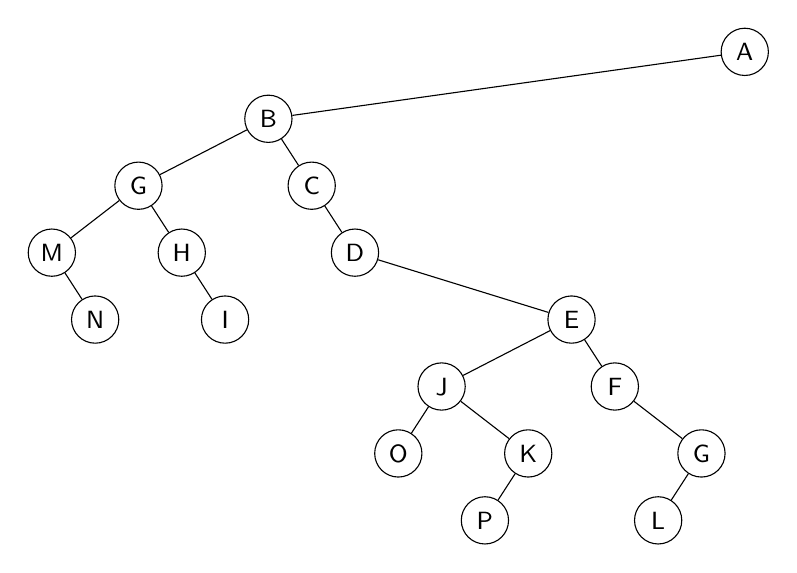
\begin{tikzpicture}[x=0.55cm,y=-0.85cm,
  every node/.style={circle,draw,minimum size=6mm,inner sep=0pt,font=\sffamily\small}]
\node (A) at (17,0) {A};
\node (B) at (6,1) {B};
\node (G2) at (3,2) {G};
\node (C) at (7,2) {C};
\node (M) at (1,3) {M};
\node (H) at (4,3) {H};
\node (D) at (8,3) {D};
\node (N) at (2,4) {N};
\node (I) at (5,4) {I};
\node (E) at (13,4) {E};
\node (J) at (10,5) {J};
\node (F) at (14,5) {F};
\node (O) at (9,6) {O};
\node (K) at (12,6) {K};
\node (G) at (16,6) {G};
\node (P) at (11,7) {P};
\node (L) at (15,7) {L};
\draw (A) -- (B) (B) -- (G2) (B) -- (C) (G2) -- (M) (G2) -- (H) (M) -- (N) (H) -- (I)
      (C) -- (D) (D) -- (E) (E) -- (J) (E) -- (F) (J) -- (O) (J) -- (K) (K) -- (P)
      (F) -- (G) (G) -- (L);
\end{tikzpicture}
\end{center}

\textbf{檢查}。 左孩子右兄弟轉出來的二元樹，前序和原來的樹的前序相同，中序和原來的樹的後序相同：
\begin{itemize}
\item 前序：A B G M N H I C D E J O K P F G L，和原樹由上而下、由左而右的前序一致；
\item 中序：M N G H I B C D O J P K E F L G A，正是原樹的後序（每個節點在它所有子孫之後）。
\end{itemize}
根 A 沒有右子節點，因為根沒有兄弟。
\end{pastsoln}
